\begin{figure*}[!tb]
  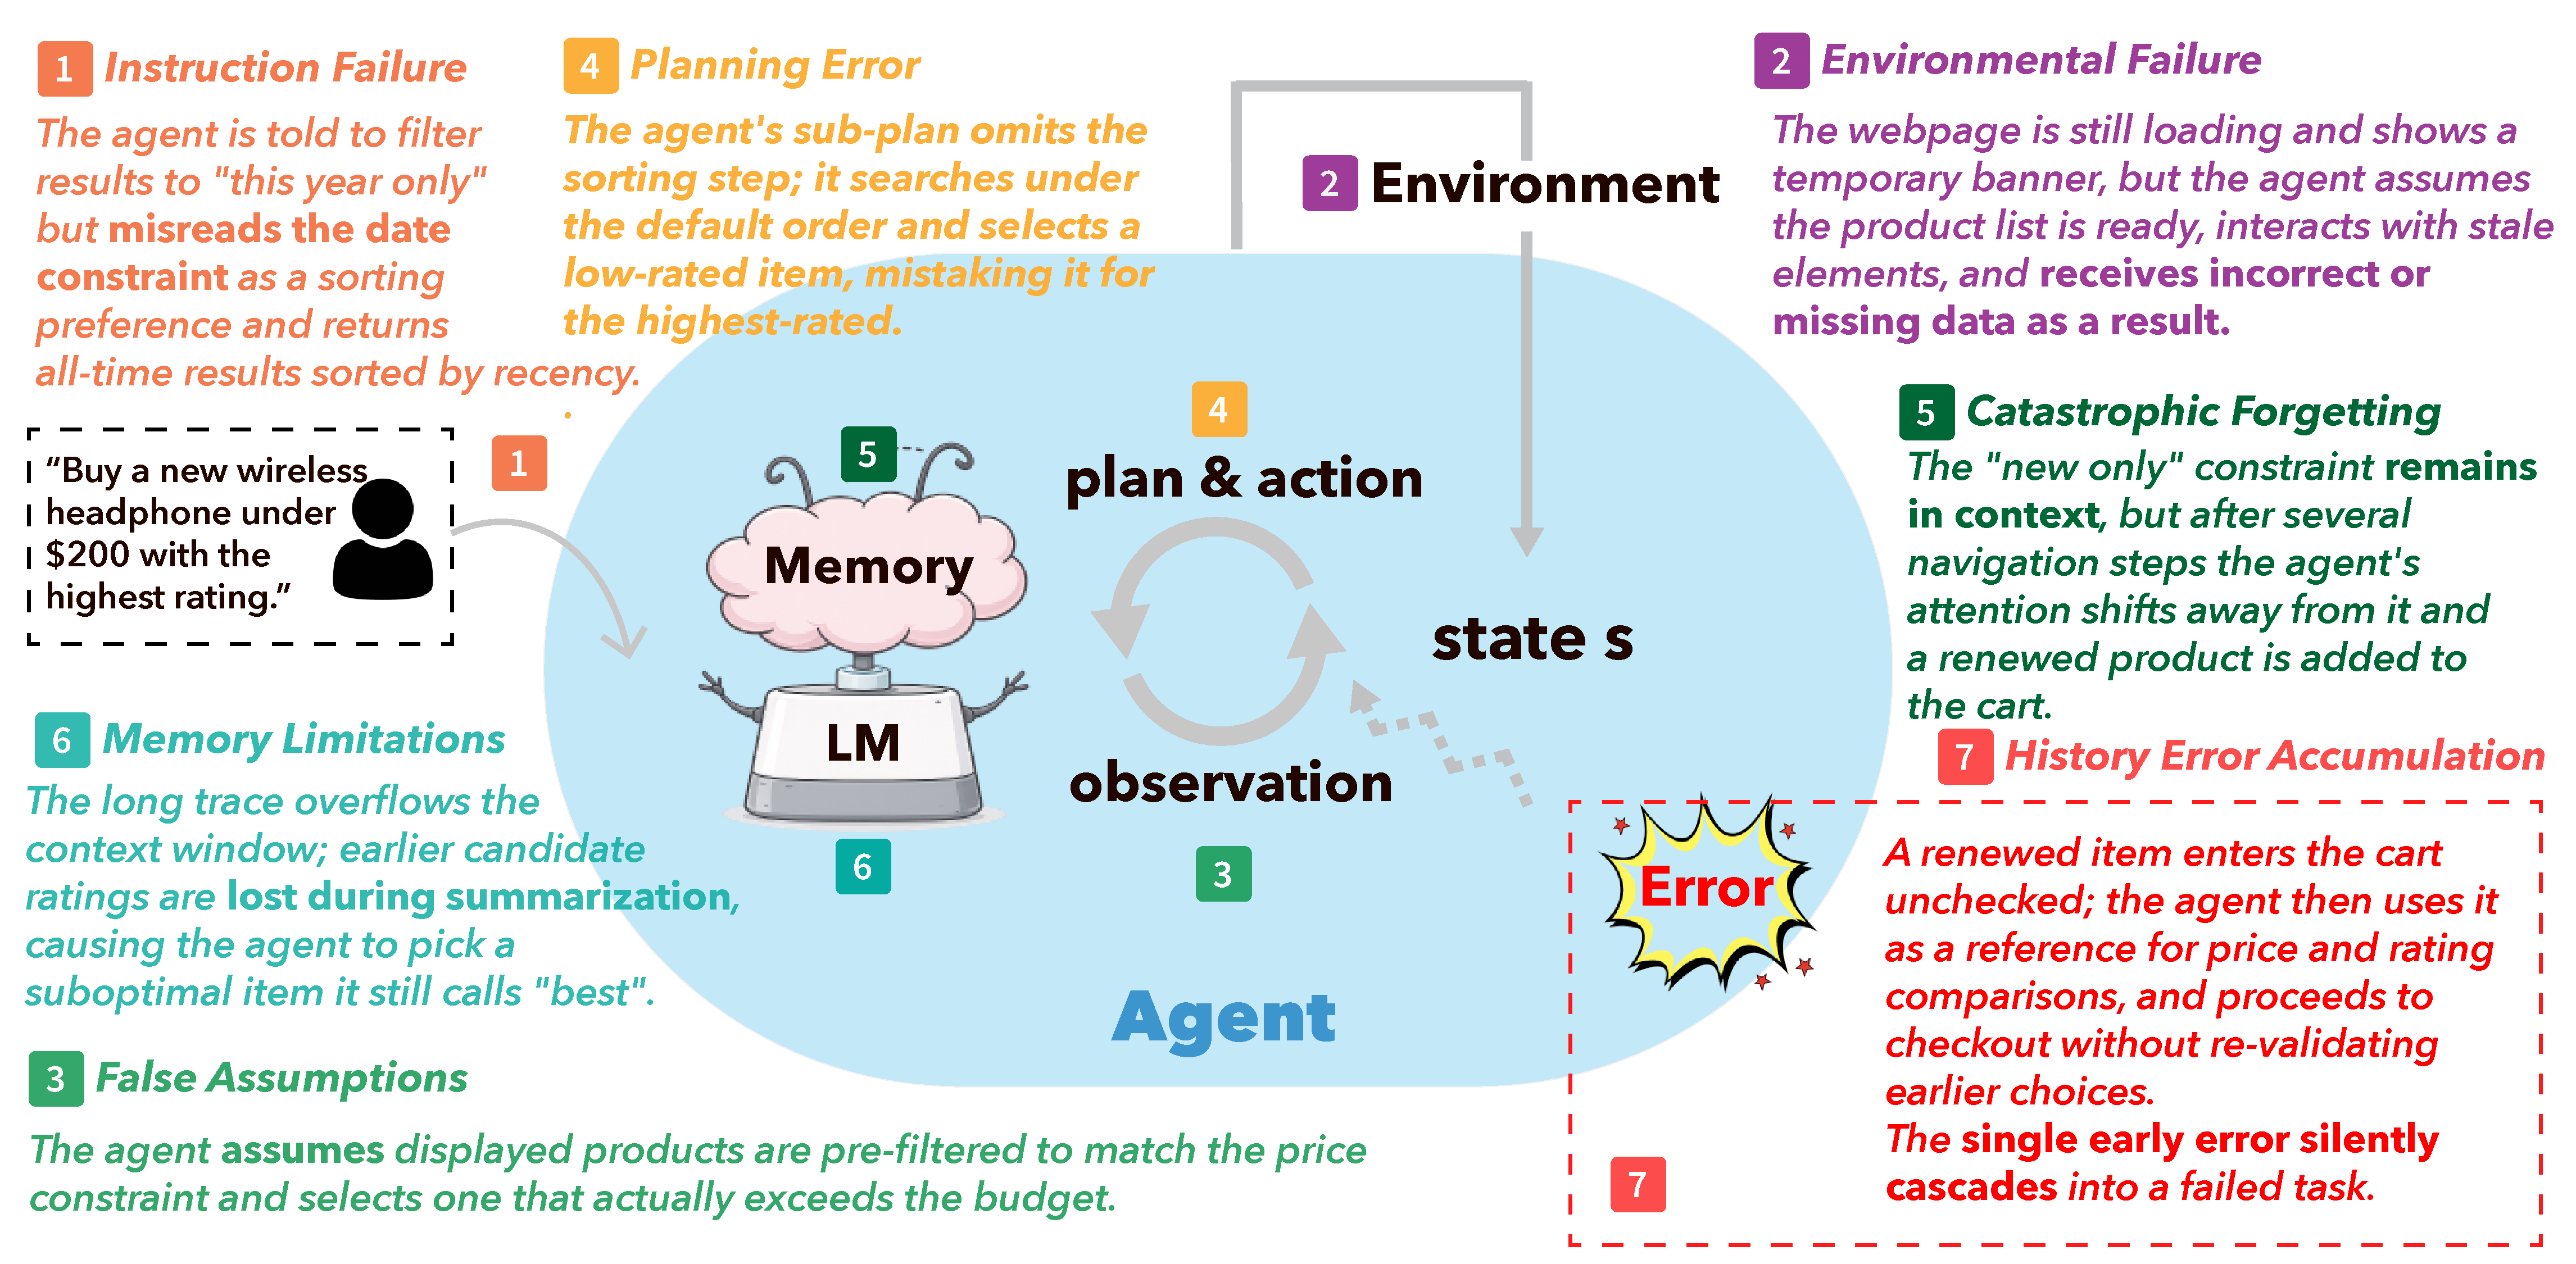
\includegraphics[width=\textwidth]{Agent.pdf}
  \centering
\caption{\textit{Illustration of general agent execution and failure propagation.}
Given an instruction \instbox, the agent iterates a standard loop:
it observes the environment \envbox to obtain observations \obsbox,
plans and selects an action \planbox drawing on memory-backed context \membox,
executes that action to change the environment,
and then updates its internal state \forgetbox through memory \membox.
Failures can originate at any stage and compound across cycles \histbox.
The seven legend boxes map directly to the failure categories in Table~\ref{tab:taxonomy_def}.}
  \label{fig:agent_failure_framework}
\end{figure*}